%
%                       This is a LaTeX 2e version of the
%                       laboratory project template file.
\documentclass[a4paper,12pt]{article}
\usepackage{fullpage,epsf}


%
%                       This section generates a title page
%                       Edit only the sections indicated to put
%                       in the project title, your name, supervisor,
%                       project length in weeks and submission date
%
\begin{document}
\pagestyle{empty}                       % No numbers of title page                      
\epsfxsize=40mm                         % Size of crest
\begin{minipage}[b]{110mm}
        {\Huge\bf School of Physics\\ and Astronomy
        \vspace*{17mm}}
\end{minipage}
\hfill
\begin{minipage}[t]{40mm}               
        \makebox[40mm]{
        \epsffile{crest.eps}}
\end{minipage}
\par\noindent                                           % Centre Title, and name
\vspace*{2cm}
\begin{center}
        \Large\bf \Large\bf Senior Honours Project\\
        \Large\bf Physics 4\\[10pt]                     % Change to MP/CP/Astro
        \LARGE\bf Template for Writing a Report         % Change to suit
\end{center}
\vspace*{0.5cm}
\begin{center}
        \bf William Hossack\\                           % Repace with your name
        October 2000                                    % Submission Date
\end{center}
\vspace*{5mm}
%
%                       Insert your abstract HERE
%                       
\begin{abstract}
        The abstract is a short, concise explanation of the project
        covering the aims, outlines of techniques used and a short
        summary of the results. It should contain enough information to
        make the aims and success of the project clear, but contain no details.
        A typical abstract should be between 50 and 100 words.
\end{abstract}

\vspace*{1cm}

\subsubsection*{Declaration}

\begin{quotation}
        I declare that this project and report is my own work.
\end{quotation}

\vspace*{2cm}
Signature:\hspace*{8cm}Date:

\vfill
{\bf Supervisor:} Dr. A.N. Other                % Change to suit
\hfill
6 Weeks                                         % Change to suit
\newpage
%
%                       End of Title Page
\pagestyle{plain}                               % Page numbers at bottom
\setcounter{page}{1}                            % Set page number to 1
\tableofcontents                                % Makes Table of Contents
%The introduction section of the report should introduce the project in
%more detail than in the abstract. In particular it should present the
%motivation, the aims, outline of techniques used, and the scope of the project. 
%It should also contain references to similar work in the
%same field to put your work in the correct context.
%
%As a general rule, people reading the abstract and introduction alone
%should have a good idea of the material in the project, the techniques
%employed and the results obtained. A typical introduction should be
%about 1 page, (300-450 words).
\section{Introduction}
%
Objectively comparing and ranking a set of entities is an important challenge. Consumers are daily tested to choose the right products, companies look for the most fruitful strategies to pursue, online search engines order query results by relevance and competitors seek to find who is the best. If there are clear criteria for comparison, ranking is straightforward. For example, marathons are always the same distance and with similar surface properties and topology. Some additional details may need to be taken into account like different age groups of the runners, but in general it is sufficient to compare the competitors' run rimes (historic or recent) in order to establish their ability.\\ 
However, not all ranking problems present clear criteria. In team sports and multi-player video games the landscape is more complicated. How do individual player contributions accumulate to reach the eventual victory or defeat? Is a team that barely wins or one that wins by a large margin better in the long run? These questions hardly have a conclusive answer. There are also added complications because people act differently depending on the nature of the competition. For instance, students in exams generally attempt to do their best without directly knowing how well their competition is doing, yet in the end it is their relative rather than absolute performance that matters most. In contrast, a marathon runner might go for their personal best, try to set a world record or just stay a few seconds ahead of their pursuer. These and other approaches reflect a person's underlying ability differently.\\
One way to approach complicated systems is to abstract away from specific details and employ statistical methods; increasing sophistication does not always produce increasingly accurate results. A ranking scheme of this type is employed by the British Orienteering Federation (BOF) to assign points to orienteering event participants. The aims of this project is to evaluate the BOF ranking scheme for accuracy and to uncover the cause of some of its quirks like the drifting of the mean of ranks over time. The problem will first be approached using computer simulated races and later the scheme will be applied to real race data.\\ 
%Theory and background
% short overview of theoretical background to project
% principles of experiment, no derivations
%Literature survery
% a review of relevant topics and work within the field (not just a list)
% some depth
% must provide added value beyond results of report
% annotated well
% avoid webpages if possible
\section{Background or Theory}
Clear criteria for arranging a group of entities in order of quality are not always available. In such cases it is desirable to infer the ranks from results of comparison events between the entities. The goal is to find each participant's skill level and to remove as much noise from it as possible. This will be referred to as skill based ranking.\\
A good starting point of skill based ranking is the Elo rating system\cite{elo}. It was developed by Arpad Elo and found its primary use in comparing chess players. The basic principle of the system is that each player's skill can be represented by a Gaussian curve. The player's skill is thought to be the mean of the curve and variation to it is allowed by the sloping sides. When two players enter a match, the likelihood if outcomes can be found by looking at the difference of both players' skill curves. The rank change of both players after the game are proportional to how unlikely that outcome was. The system has been applied to other sports as well, for example football\cite{football}.\\
A weakness of the Elo system is that it assigns an equal uncertainty to all players' ranks, this is addressed in the Glicko system\cite{glicko}. In this system a person who plays frequently is subject to smaller rank changes than someone who plays less frequently. As a player accumulates more and consistent games, the standard deviation around their mean rank shrinks.\\
A further extension to include multiplayer games is Microsoft's TrueSkill which was developed for the Xbox gaming system\cite{trueskill}. The principle is very similar to Glicko, expected outcomes leave ranks almost unchanged while upsets cause big changes. Teams of players are assigned aggregate mean skill and uncertainty, the outcome of the match usually causes different individual rank changes for each player. Where more than two teams or players are competing all against each other, the participating entities are compared pairwise. The system also includes iterative steps that run the same scores through the system multiple times and different weights for game types based on how big of a role luck and skill plays. The exact details of the algorithm are rather involved and excellent explanations and a sample implementation can be found in other resources(\cite{trueskillMicrosoft}, \cite{trueskillSimple}). This ranking system has an elaborate theoretical basis and has shown good predictive power\cite{trueskill}. An interesting expansion of TrueSkill is AllegSkill\cite{allegskill} where additional provision exists for team commanders' skills.\\
A shared feature of the discussed ranking systems is that they are geared towards evaluation one versus one competitions. While all versus all ranking applications are possible, in practice they are executed as a series of one versus one comparisons. The ranking scheme used by British Orienteering Federation, the focus of this report, is an all versus all system in essence. The central equation of interest is the score assignment formula\cite{bof}:
\begin{equation}
RP = MP + \frac{SP * (MT - RT)}{ST}
\label{eq:mainEq}
\end{equation}
Where R stands for run, P for points, T for time, M for mean and S for standard deviation. The formula says that the number of points awarded to a runner in a race is the mean number of points of the runners participating in that race plus the standard deviation of the runners' points multiplied by the number of standard deviation that the runner being awarded is away from the mean time of all runners' times. The best guess of a runner's skill is the mean of their scores obtained races (published scores usually the mean of a subset of all scores).\\
It is tempting to include in the discussion the central limit theorem (CLT) which states that the distribution of means sampled from almost any distribution will tend to a Gaussian\cite{probability}. However, the theorem requires independent samples drawn from an identical distribution. When ranking, samples are being essentially from the distribution of abilities. Complications are added by the fact that this distribution changes over time and samples some times correlate if runners interact. Also, the ability is interpreted via the score assignment formula and is not drawn directly. Thus, while the CLT might apply in some states, in general it is difficult to rigorously apply it to this system.\\
Another concept that must be mentioned is self consistency. One application of this principle is the Hartree-Fock algorithm. In the method a trial wavefunction is used to calculate the energy of a complicated quantum system. This energy is then used to adjust free variables in the wavefunction, which is then used again to gain a new estimate of the energy. The loop is continued until new approximations do not appreciably change. The system has then then reached self consistency. This principle could be applied to orienteering ranking by putting race results back though the system multiple times, each time potentially improving the estimate of the players' ranks. It would be reassuring if the system eventually settled on a stable state instead of changing ranks continually.\\
Because systems similar to the one used by the British Orienteering Federation are not widely discussed in scientific literature, an approach based on simulations and experiments will be used to analyze the ranking scheme.
%Description of
% apparatus (code) and how it works
% experimental method and procedures
% calibration(?)

%Scope
% enough to allow th reader to udnerstand how the experiment was carried out
% very important that for people attempting to reproduce your results

%Useful tips
% diagrams!
% reference borrowed figures

%This section should contain the details of the method employed. 
%As in the previous sections standard techniques should not be written
%out in detail. For example if you use an oscilloscope to take a
%measurement, the theory of the CRO tube\footnote{Don't laugh, I have actually
%seen this.} is {\bf not relevant}. In computational projects this
%section should be used to explain the algorithms used and the layout of
%the computational code. A copy of the acutal code must be
%given in the appendices. Long detailed sections of theory, data tables
%and details of computational code used in data analysis only should not
%appear in this section, but should/may be included in the appendices.
%
%This section should emphasise the philosophy of the approach used
%and detail novel techniques. However
%please note: this section in {\bf not} a blow-by-blow account of what
%you did throughout the project, and in particular it should {\bf not} 
%contain large detailed sections about things you tried and found to be
%completely wrong. Remember you are writing a technical report, and
%not a diary. If however you find that a technique that was expected to
%work failed, that is a valid result and should be included.
%
%Here logical structure is particularly important, and you may find that
%to maintain good structure you may have to present the experiments
%in a different order from the one in which you carried them out.

\section{Method or Strategy}
All simulations and analysis scripts are implemented in Python 2.7. The Numpy library is used for certain numerical tasks and Pyplot is used for plots and histograms. Most of the data analysis functions are implemented in a separate module. The main script then calls them in order according to user-defined control variables. (see SOME APPENDINX for implementation)

\subsection{Simulation}
All simulation code follows the following pattern.
\begin{itemize}
\item Create a collection of runners and assign initial scores.
\item (optional) Assign each runner ability.
\item Execute the following update loop m times:
	\begin{enumerate}
	\item Select a group of runners from the whole list.
	\item Generate run times.
	\item (optional) Mark slowest 10\% to be excluded from calculations.
	\item Calculate and apply score changes as per formula [???].
	\end{enumerate}
\end{itemize}

Two types of score initialization were considered: all starting from the same score of a 1000 or assign scores based on a a Gaussian peaking at 1000 and with standard deviation of 200. In the case of uniform score assignment care needs to be taken in the code to handle the case when SP is zero (all runners have the same score) leading to division by zero.\\
The code was progressively expanded to add more details about the runners. Initially there was no distinction between the competitors, later each runner was assigned an intrinsic ability and variability of that ability. The underlying ability distribution is modeled as each runner having a mean time. In reality, courses have different lengths, hence they take a different time to complete. The model used here corresponds to different subsets of all competitors running the same track in their own mean time. This should not be an issue because run times are essentially normalized when scores are calculated because only deviations from the mean time are relevant.
In the case of no innate ability, run times are generated from a Gaussian curve with a random mean and standard deviation as one tenth of that mean.\\ 
The variability of a runner's performance is represented by a mean number of mistakes they make in a race. Every time they compete, a Poisson random variable with a mean of that runner's specific number of mistakes is drawn. This is multiplied by a mistake weight factor and added to their run time. [+- mistakes as well...]

\subsection{Analysis of Real Data}
A pre-processing step was performed to speed up subsequent data processing. Outside of the main program, incomplete entries were removed it would not be possible to gain information from them later.\\
The main script follows the following pattern.
\begin{itemize}
\item Process the data file and produce a list of races and a list of all participants.
\item Assign runners initial scores.
\item For each race in the list of all recorded races:
	\begin{enumerate}
	\item (optional) Identify and deal with outliers.
	\item Calculate and apply score changes as per formula [???].
	\end{enumerate}
\end{itemize}
The file processing step parses the input CSV (comma separated values) file and assembles a list of races where each race is a list of a participant, run time pairs. In order to conform to the BOF rules, some data is discarded at this stage if the course is of type "yellow" or "white", if the participant is under the age of 16 or if the race has less than 10 participants. Also, run times that are 0 seconds long are discarded as they are obvious errors in recording. Still, other less-clear outliers remain.\\
Initial scores, same as before, can either be some constant value for everyone or a normally distributed random variable.\\
Possible outliers can be identified as either the slowest 10\% or times that are some number of standard deviations away from the mean of all times. They can then be either excluded from calculations of MT, ST, MP and SP or removed altogether giving them no points for the race.

\subsection{Reruns}
It is also possible to run all scores through the score assignment system multiple times. This would ideally lead to decreasing rank adjustments each rerun as the players' true score becomes better approximated each cycle.  
%Description of
% analysis proccedures and error propogation (enough info to test your results)
% code and data processing stuff
% errorr barrrs
% plots of residuals when fitting to data
%Assumptions and approximations
%error analysis
% comparison of results with lit vals
%significance and relevance of results
%consistency of data, limitations, improvements
%This section should detail the obtained results in a clear,
%easy-to-follow manner. Remember long tables of numbers are just as boring to
%read as they are to type-in. Use graphs to present your results where
%-ever practicable. When quoting results or measurements
%{\bf DO NOT FORGET ABOUT ERRORS}. Remember there are two basic types
%of errors, these being random and systematic, which you must consider.
%Remember also the difference between an error and a mistake, computer
%program bugs are mistakes.
%
% 
%Again be selective in what you include. Half a dozen
%tables that contain totally wrong data you collected while you forgot
%to switch on the power supply are {\bf not relevant} and will frequently
%mask the correct results. 
%%
%%                       Here is how to inserted a centered
%%                       postscript file, this one is actually
%%                       out of Maple, but it will work for other
%%                       figures out of Xfig, Idraw and Xgraph
%%
%\begin{figure}[htb]     %Insert a figure as soon as possible
%        \begin{center}
%                \leavevmode             % Warn Latex a figure is comming
%                \epsfxsize=90mm         % Horizontal size YOU want
%                                        % figure to be
%                \epsffile{./images/otf.eps}
%\end{center}
%\caption{This is an inserted Postscript file}
%\end{figure}
%
%This section must contain a discussion of the results. This should
%include a discussion of the experimental and/or numerical errors, and a
%comparison with the predictions of the background and theory underlying
%the techniques used. This section should highlight particular strengths
%and/or weaknesses of the methods used.
\section{Results and Discussion}
\subsection{Simulation results}
The first simulated case is that of there being no difference between the runners (see Fig \ref{fig:sameAbilitiesRanks}). The general trend observed here was that the participants' final rank distribution is described by a sharply peaked curve with the mean matching the one of the initial rank distribution's mean. This was expected because the runners have no intrinsic ability and their race times are generated at random. Over time the ranking scheme is able to deduce that all runners have the same skill level, despite being assigned different initial ranks. As the number of races increases, the system becomes more certain of this result, which is reflected by the peak becoming sharp.
%As more races are executed, the standard deviation of the ranks becomes smaller (Fig \ref{fig:sameAbilitiesRanksStds}).
\begin{figure}[h]     
\begin{center}
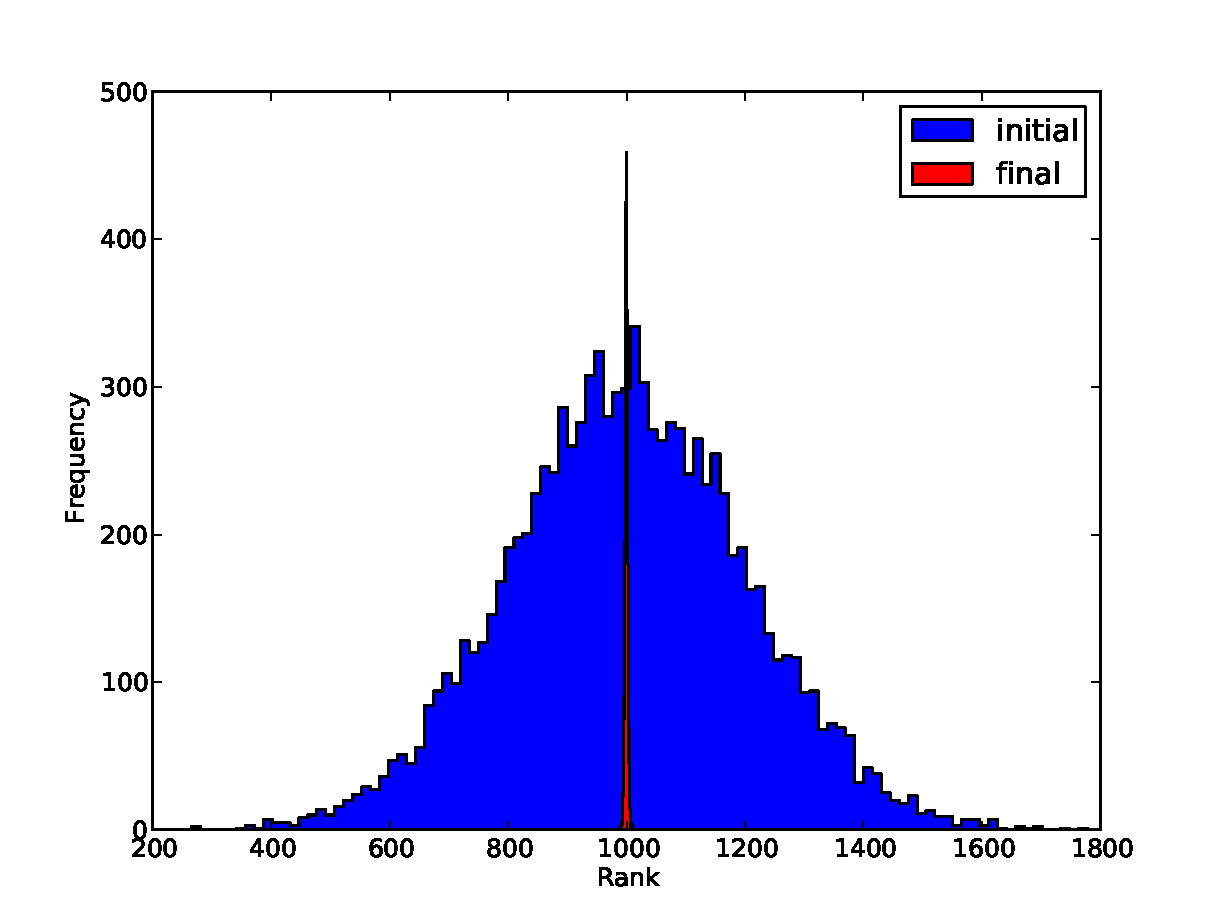
\includegraphics[width=15cm]{./images/sameAbilitiesRanks.pdf}
\end{center}
\caption{Rank histogram of initial ranks and final ranks for runners with no intrinsic ability. Initial $\mu=1000$ and $\sigma=200$, final $\mu=1000$ and $\sigma=2$; 30000 races in total. Note: bin widths are different for the two histograms.}
\label{fig:sameAbilitiesRanks}
\end{figure}\\
%\begin{figure}[h]     
%	\begin{center}
%    	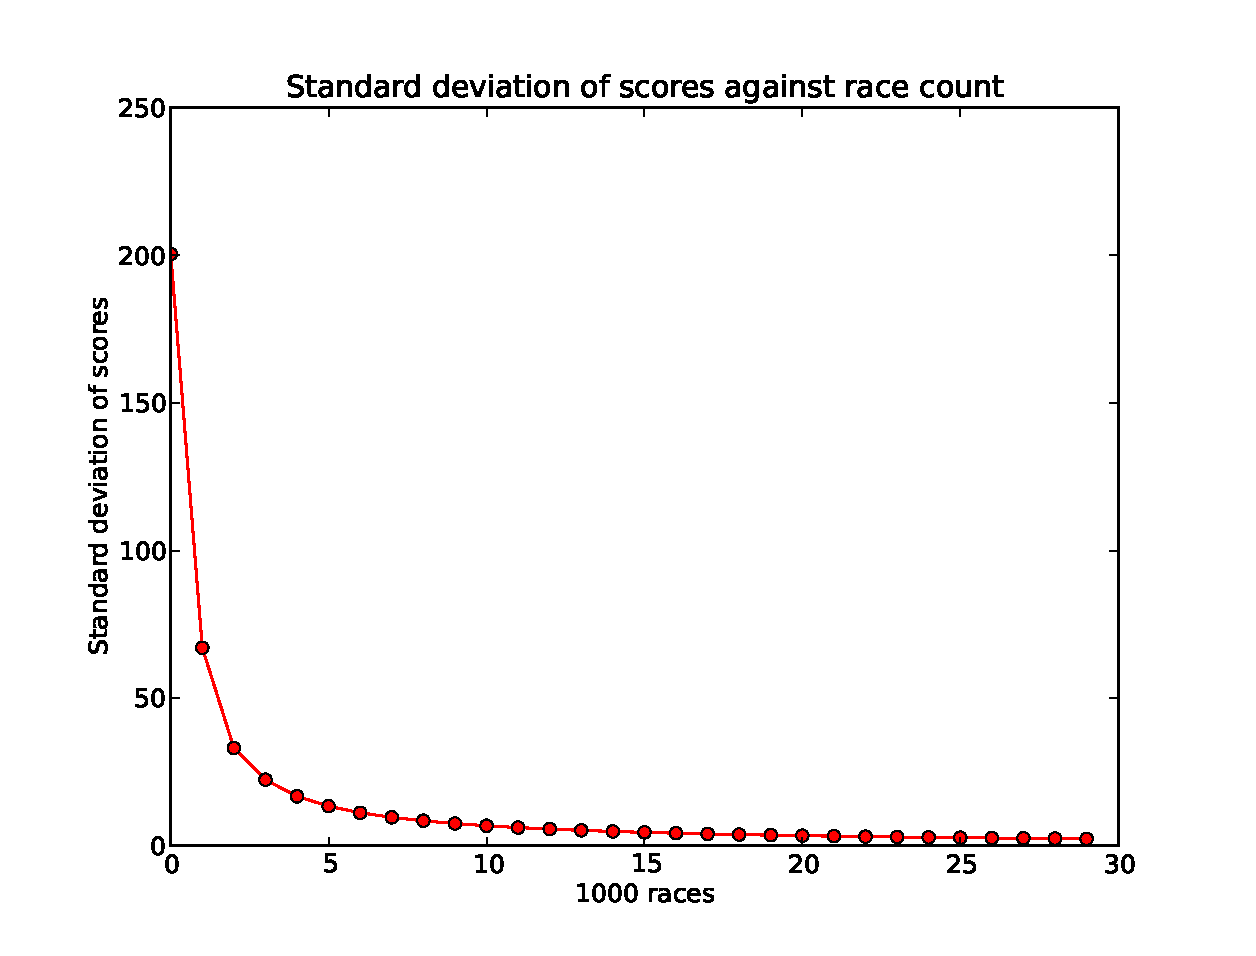
\includegraphics[width=15cm]{./images/sameAbilitiesRanksStds.eps}
%	\end{center}
%	\caption{Standard deviation of means against race count for runners with no intrinsic ability.}
%	\label{fig:sameAbilitiesRanksStds}
%\end{figure}
Next, the 90\% cutoff rule was applied. It was observed that the rule produced a large drift (156 points) of the mean to the left, i.e. in the negative direction (see Fig \ref{fig:meanDrift}). The drift levels off as standard deviation decreases due to increasing sampling. The underlying cause was identified to be giving points to runners that were beyond the cutoff point. Removing the longest 10\% of run times for calculations of \emph{MT}, \emph{ST}, \emph{MP} and \emph{ST} while still giving points to the excluded runners creates a bias towards the lower scores. The mean run time is artificially lowered which leads to the excluded players receiving an inappropriately lower score which in turn leads to the whole rank distribution to drift to the left over time. Applying the same cutoff rule but this time not giving points to the excluded produced the same results as in Figure \ref{fig:sameAbilitiesRanks}.
%The decrease levels off as the standard deviation of the scores becomes smaller.
\begin{figure}[h]     
    \begin{center}                        
        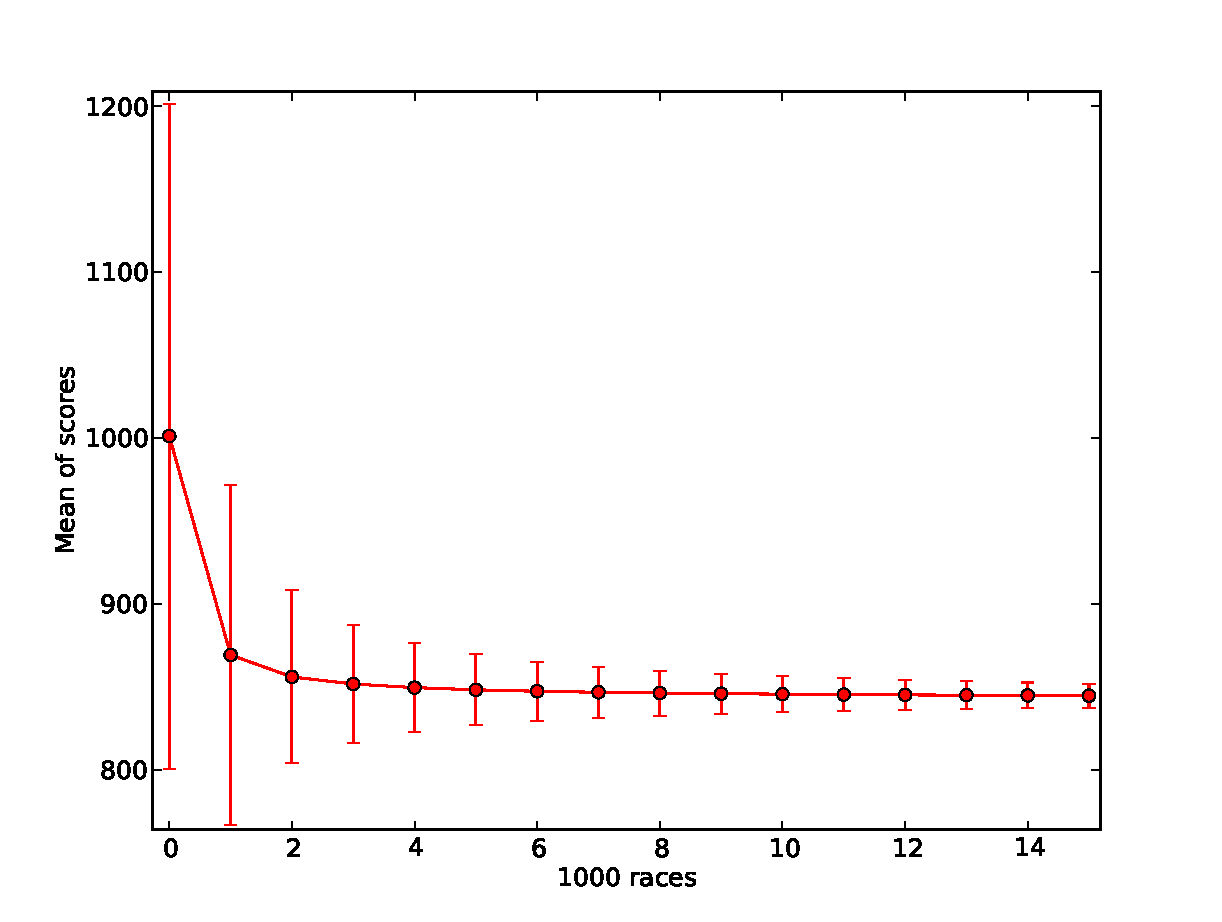
\includegraphics[width=15cm]{./images/meanDrift.pdf}
	\end{center}
	\caption{Mean of scores against race count for runners with no intrinsic ability. Initial $\mu=1000$ and $\sigma=200$. The 90\% cutoff rule is applied. Error bars show standard deviation.}
	\label{fig:meanDrift}
\end{figure}\\
Runners with differing intrinsic abilities (see section \ref{sec:method} for implementation details) were put through the system next. To present the comparison between the runners' innate abilities and the rank assigned to them by the system, plots of these two quantities against each other are used. For a successful ranking attempt it is expected to see a straight line with a negative slope (higher mean run time corresponds to lower skill). If the runners make no mistakes, the system was found to correctly identify runners' abilities. Both Gaussian and constant initialization produced the correct plot showing that the system identified runners' intrinsic abilities correctly. However, with constant initialization some data (about 3\%) have a comparatively high standard deviation(see Fig \ref{fig:diffAbilitiesNoErrorConstantInit}). Examining these data points revealed that they usually have one race early on that produced a distant outlier, probably by putting them in a poorly matched race. Rerunning the simulation with the previously estimated ranks as the new initial ranks removed all outliers and produced consistent, small standard deviations. It is interesting that this effect did not arise when the system was initialized with Gaussian ranks. This was probably caused by initial "smoothing" of \emph{SP} so that very good runs did not earn an unreasonably high amount of points. These results inspire confidence that the code is correct.
%\begin{figure}[h]     
%    \begin{center}                        
%        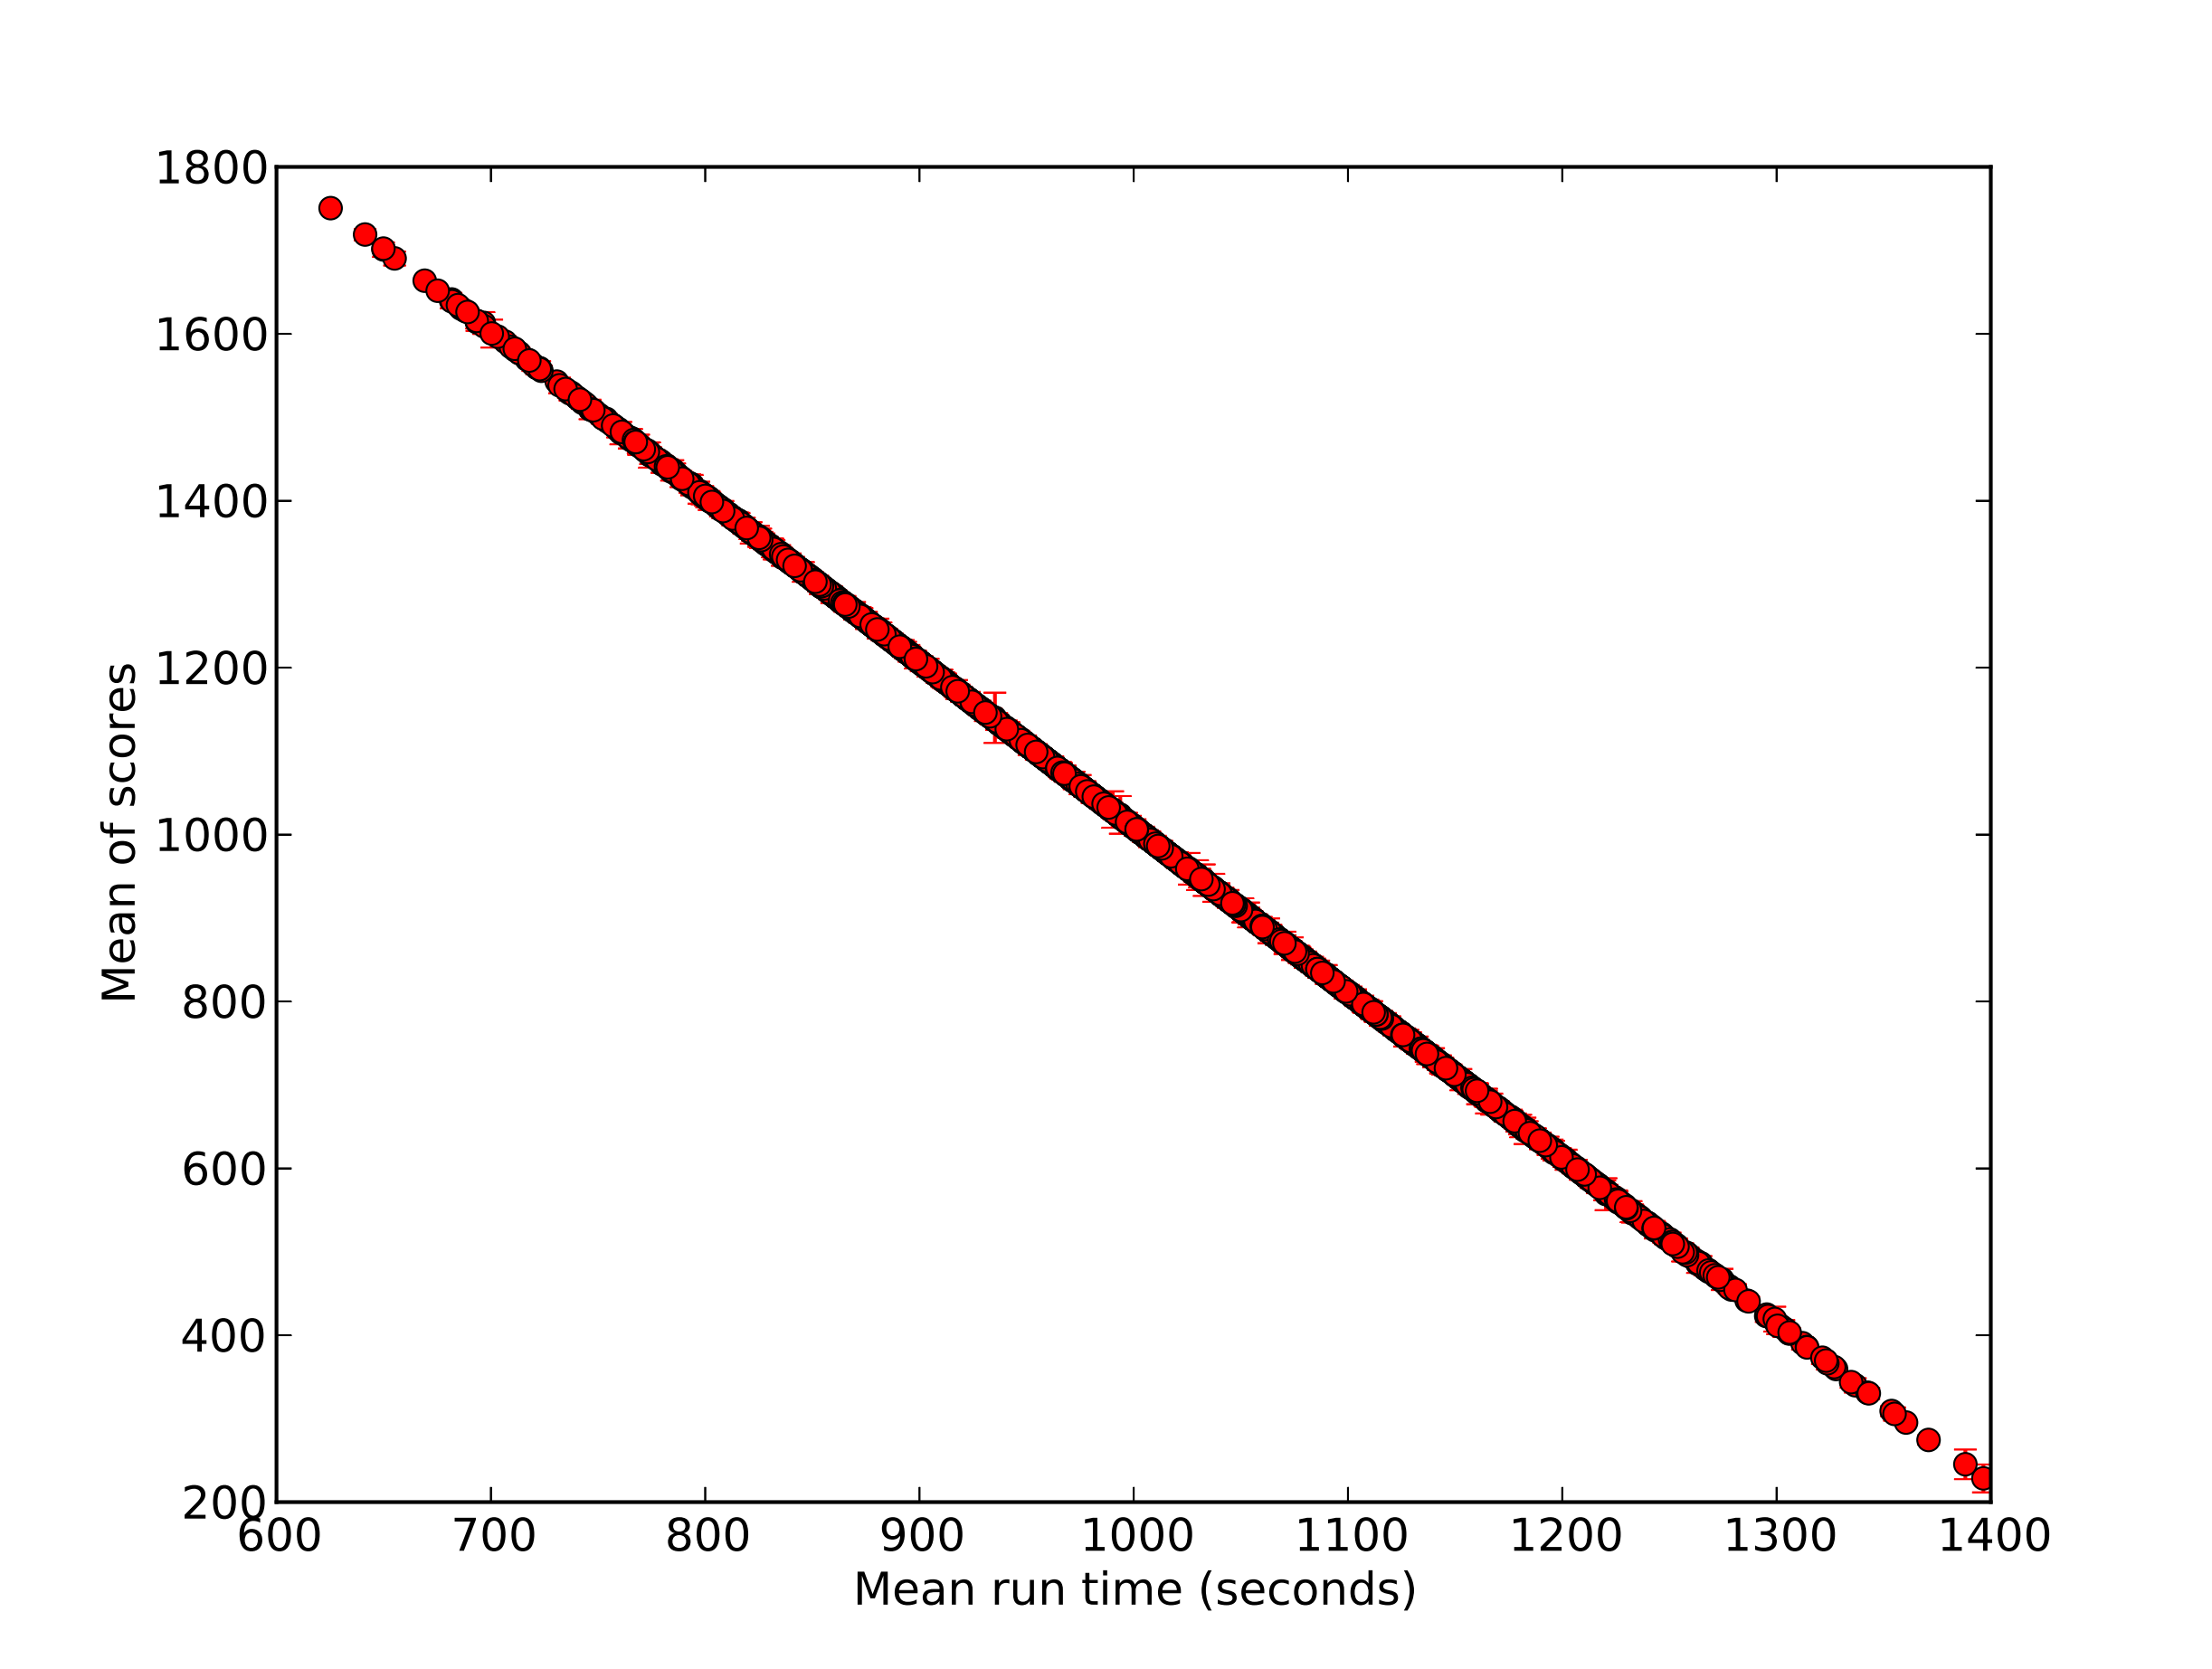
\includegraphics[width=15cm]{./images/diffAbilitiesNoErrorNormalInit.png}
%	\end{center}
%	\caption{Mean of awarded scores plotted against mean run time(ability). Initial ranks were distributed from a Gaussian with $\mu=1000$ and $\sigma=200$. Final ranks have $\mu=1006$ and $\sigma=199$. Error bars show standard deviation, standard errors are too small to see.}
%	\label{fig:diffAbilitiesNoErrorNormalInit}
%\end{figure}
\begin{figure}[h]     
    \begin{center}                        
        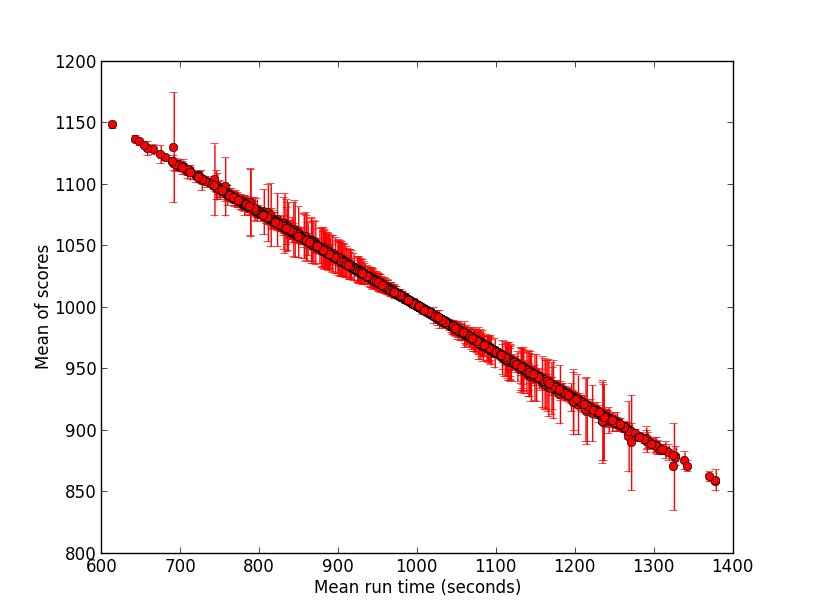
\includegraphics[width=15cm]{./images/diffAbilitiesNoErrorConstantInit.png}
	\end{center}
	\caption{Mean of awarded scores plotted against mean run time. Initial ranks were all 1000. Final ranks have $\mu=1000$ and $\sigma=38$; 30000 races in total. Error bars show standard deviation, standard errors are too small to see. Points with high standard deviation represent about 3\% of the data.}
	\label{fig:diffAbilitiesNoErrorConstantInit}
\end{figure}\\
Adding in running mistakes, i.e. increasing noise, makes it more difficult to distinguish runners. The rank-ability plot bulges out and data points have high standard deviation (Fig \ref{fig:doubleFigure}a). Still, the general linear shape is retained so runners with significantly different abilities are correctly ranked with respect to each other. Increasing the number of races improves the ordering of runners, as one might expect, but the noise remains (Fig \ref{fig:doubleFigure}b). Interestingly, if the initial ranks were set to correctly reflect the runners' abilities, the rank-ability plot still bulged out as before.\\
%thus the initial conditions do not have a lasting effect on the final rankings
%Giving each runner a different capacity for making mistakes had little effect, the overall impact evens out.\\ 
Rerunning the same data multiple times while keeping the total number of races the same did not improve runner rank estimation. This can be explained by noting that generating unique races creates new information and thus improves the estimate of the mean. It was noted that the standard deviation of ranks would shrink when rerunning the same sequence of races multiple times. To explore this effect, runners with no mistakes were looped 10 times with 5000 races each loop. The mean and standard deviation of scores leveled off at 1000 and 38 respectively while the mean of standard deviations of individual racers' scores went to 0. The mean and individual deviations thus behaved correctly. It is unclear why the rank deviation went to 38 rather than 100 which was the standard deviation of the abilities but at least it was correctly identified that all runners are not the same.\\
To continue, runners with error making capability were run through 10 loops of 5000 races each as well. The mean of ranks remained at 1000 but both rank standard deviation and individual standard deviations approached 0. To examine this, the scores were rebased after every run except the last one to have mean 1000 and standard deviation 200. Now the standard deviation of ranks went to 90 and that of individual scores to 85, but increasing the number of races in each loop made these fall further. This indicates that all rebasing does is reset the initial standard deviation which then falls to where it intends to be. Different settings showed similar results.\\
It is unclear what exactly is causing the shrinking distribution. It seems to echo the Central Limit Theorem which, for a simple case like averaging coin tosses, would predict that the mean of averages would converge to a sharp peak. This, however, does not fully explain (i) why the case with no mistakes levels off a $\sigma=38$ instead of the standard distribution of the abilities(100) and (ii) why introducing even a small mistake propensity makes the distribution of scores shrink. Still, the rank-ability plots do not change qualitatively so the ordering of players, which is the ultimate goal, is not impeded. For practical reasons, though, it is desirable to rebase scores between reruns as doing so when the standard deviation falls very low can be difficult due to division by a very small number.
%In this case, however, the intermediate distributions of points being drawn from
\begin{figure}[h]     
    \begin{center} 
    	\begin{subfigure}{0.49\textwidth}                       
        	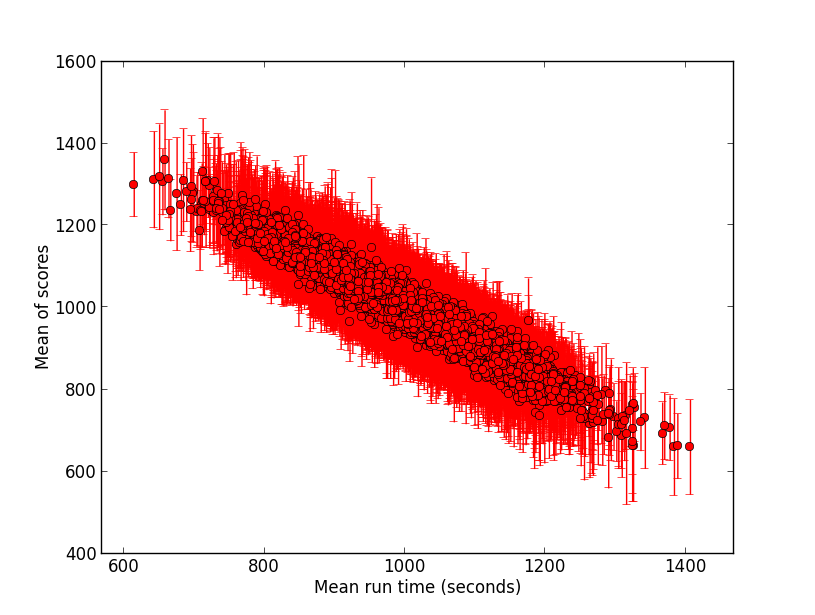
\includegraphics[width=\textwidth]{./images/diffAbilities10errorsGaussConstantInit3k.png}
        	\caption{3k races}
        \end{subfigure}
%        \begin{subfigure}{0.3\textwidth}                       
%        	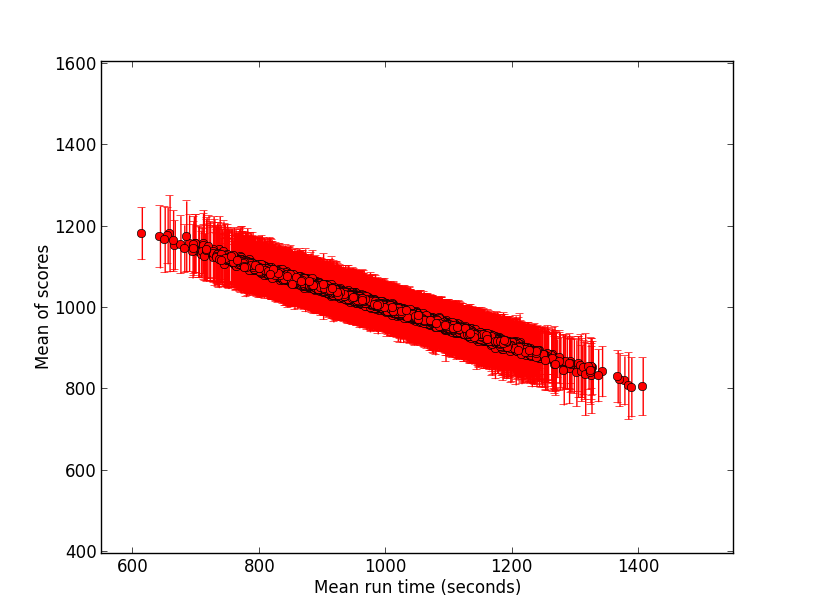
\includegraphics[width=\textwidth]{./images/diffAbilities10errorsGaussConstantInit30k.png}
%        \end{subfigure}
        \begin{subfigure}{0.49\textwidth}                       
        	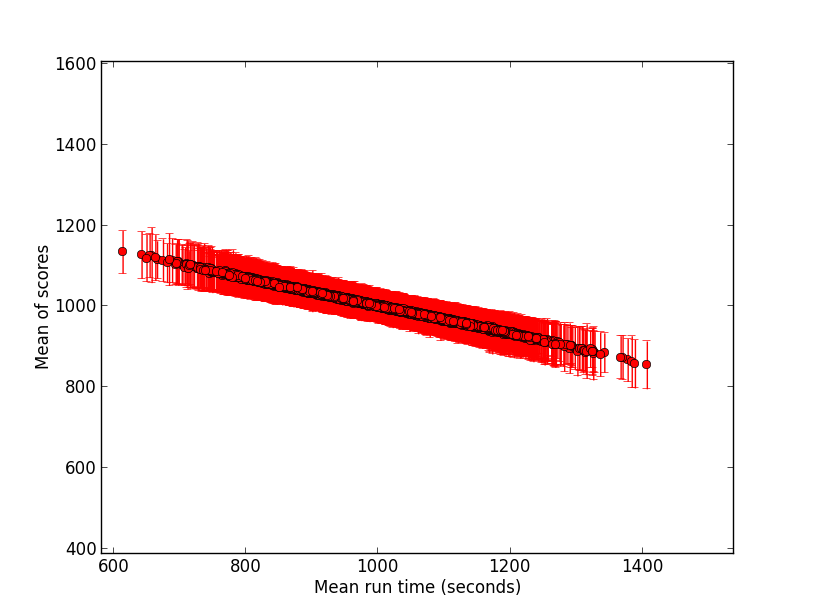
\includegraphics[width=\textwidth]{./images/diffAbilities10errorsGaussConstantInit100k.png}
        	\caption{100k races}
        \end{subfigure}
	\end{center}
	\caption{Mean of awarded scores plotted against mean run time for 2 different numbers of total races. Initial ranks were distributed from a Gaussian with $\mu=1000$ and $\sigma=200$. Final ranks have (a) $\mu=1000$ and $\sigma=92$ and (b) $\mu=1000$ and $\sigma=34$. Error bars show standard deviation, standard errors are too small to see.}
	\label{fig:doubleFigure}
\end{figure}\\
%
\FloatBarrier
\subsection{Data analysis results}
To get an idea of what the rank distribution should look like, raw race time data was analyzed. For every race time its distance in standard deviations from the mean of that particular race was calculated. The resulting distribution can be seen in Figure \ref{fig:timeDeviationDistribution}. It has a tail on the negative side which corresponds to race times that are larger than the mean. This is intuitive as achieving a very fast run is difficult while there is essentially no limit to how slow a race can be done. It is reasonable to expect that the rank distribution would have a similar shape.\\
Taking some of the observations from simulated data, a first look at the real Orienteering data was performed. The 90\% cutoff rule was not applied as it causes the distribution to drift significantly over time. Another concern with real data is poor sampling of some individuals. In the simulations runners were entered into races at random so with enough total races everyone was sampled well. In reality people have different levels of motivation, some participate frequently while others give up after one race. Both would be entered into the database. Thus in the final rank distribution only racers that have participated in 6 or more events were included. This choice was made arbitrarily to match the the fact that published scores are often the means of a runners' best 6 scores. Figure \ref{fig:simpleRealData} shows the resulting rank distributions. The data was initialized from a Gaussian an was run through twice to reduce the effect of initialization. The ranks display the same tail as the time deviation data as hoped. The fall on the right side is not as fast as that of the the time data. This could be due to only taking better sampled people into account who could be expected to perform better overall than the average due to practice.\\
Unfortunately, the shrinking of the distribution problem persisted here as with the simulated data. Repeated runs through the data caused the standard deviation of scores to fall each rerun without an obvious non-zero lower limit. Rebasing the scores between runs did not appear to improve the situation. This remains an unresolved problem and properties of convergence are unclear. Nevertheless, similarity between the time deviation and rank distributions and the earlier results from simulated data provide evidence that the people are still ranked as correctly as possible given limited data.\\
\begin{figure}[h]     
    \begin{center}                        
        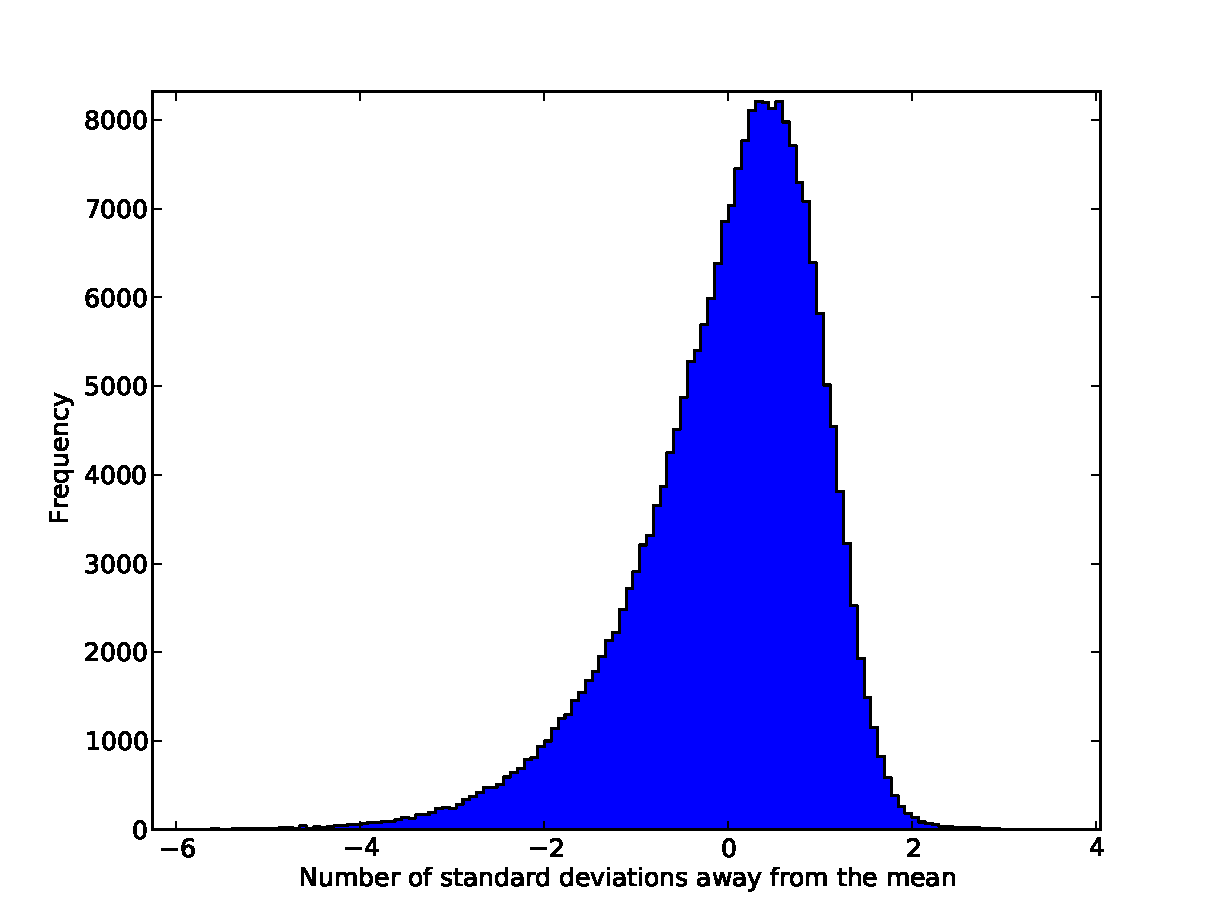
\includegraphics[width=15cm]{./images/timeDeviationDistribution.pdf}
	\end{center}
	\caption{Distribution of all run time deviations obtained from real data. $\mu=0$ and $\sigma=1$. Negative deviation corresponds to race times that are larger than the mean.}
	\label{fig:timeDeviationDistribution}
\end{figure}
\begin{figure}[h]     
    \begin{center}                        
        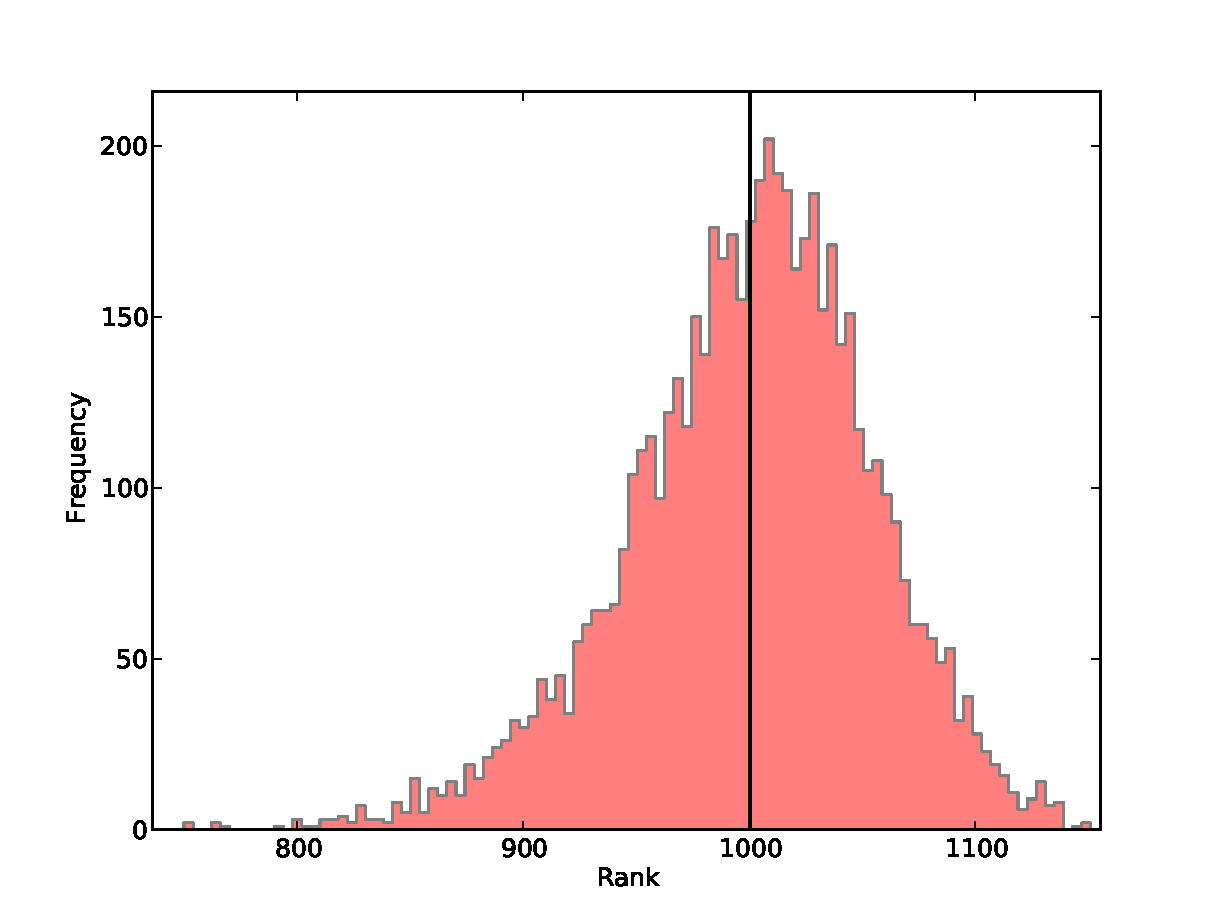
\includegraphics[width=15cm]{./images/simpleRealData.pdf}
	\end{center}
	\caption{Rank histogram for real data with 2 different. Initial ranks were Gaussian with $\mu=1000$ and $\sigma=200$. The data was run through twice. Only people who participated in 6 or more races are shown. Final ranks have (a) $\mu=1000$ and $\sigma=55$. The black vertical line marks the mean.}
	\label{fig:simpleRealData}
\end{figure}
%In both cases the distributions have tails on the low rank side as expected. Constant initialization produces a smoother distribution than Gaussian initialization but it also produces distant outliers. Similarly as before, these runners were found to have a particularly low or high first few scores that biased their mean score. However, rerunning the the data again with the improved initial scores did not remove these outliers as was the case for simulated data. This suggests that the bad scores are based on actually outlying run times. To address this, a Gaussian cutoff rule was applied that ignores run times more than 2$\sigma$ outside the mean. Applying this rule and 2 runs through the data removed the high point outlier but the low ones remained. The outliers on the low end kept changing so it appears that there truly are some poor runners that belong there. However, the outlier at the top was the same person and it was observed that none of their runs were eliminated by the cutoff, but the initial high score disappeared still. Thus it can be concluded that the high outlier was caused by someone else's anomalous run time.
%\begin{figure}[H!]     
%    \begin{center} 
%    	\begin{subfigure}{0.49\textwidth}                       
%        	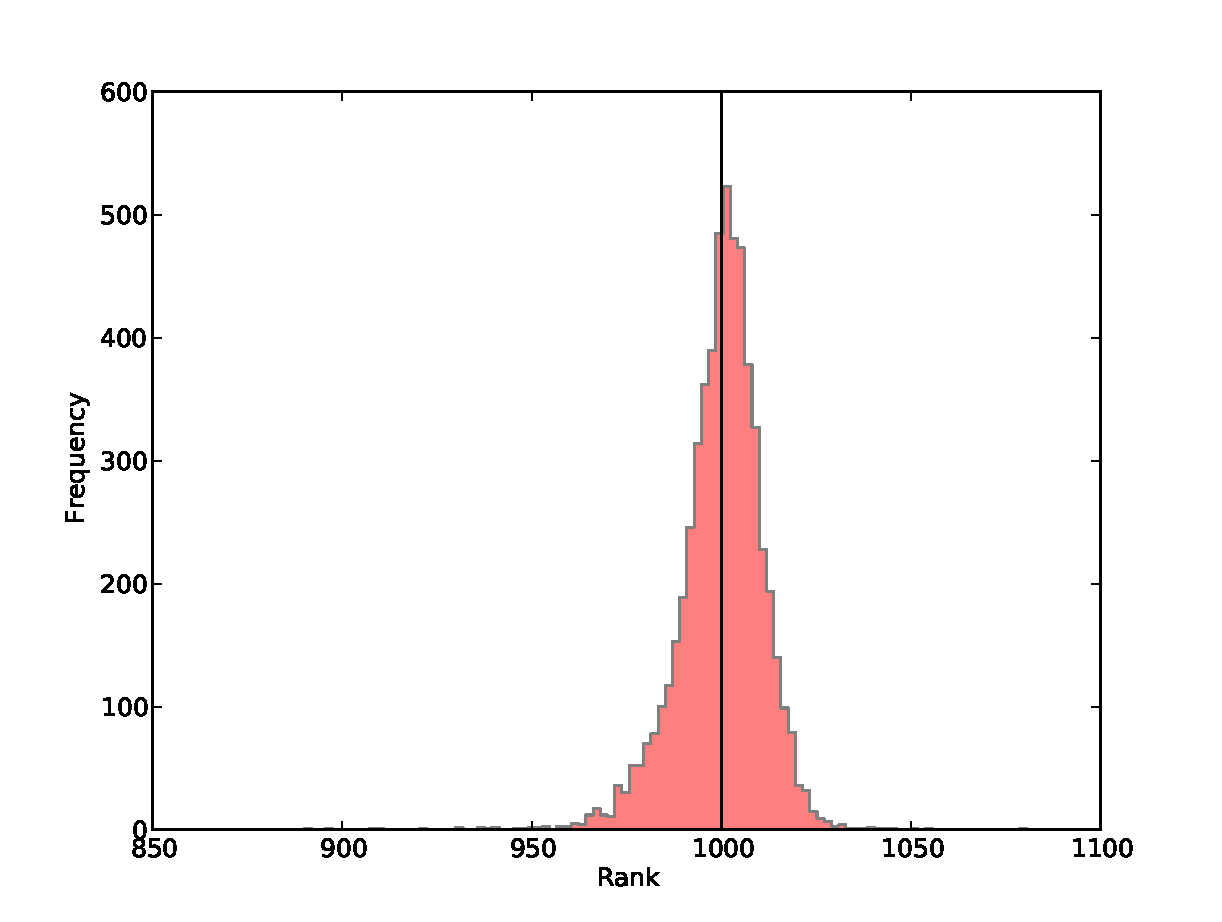
\includegraphics[width=\textwidth]{./images/realFirstLookConstant.pdf}
%        	\caption{•}
%        \end{subfigure}
%        \begin{subfigure}{0.49\textwidth}                       
%        	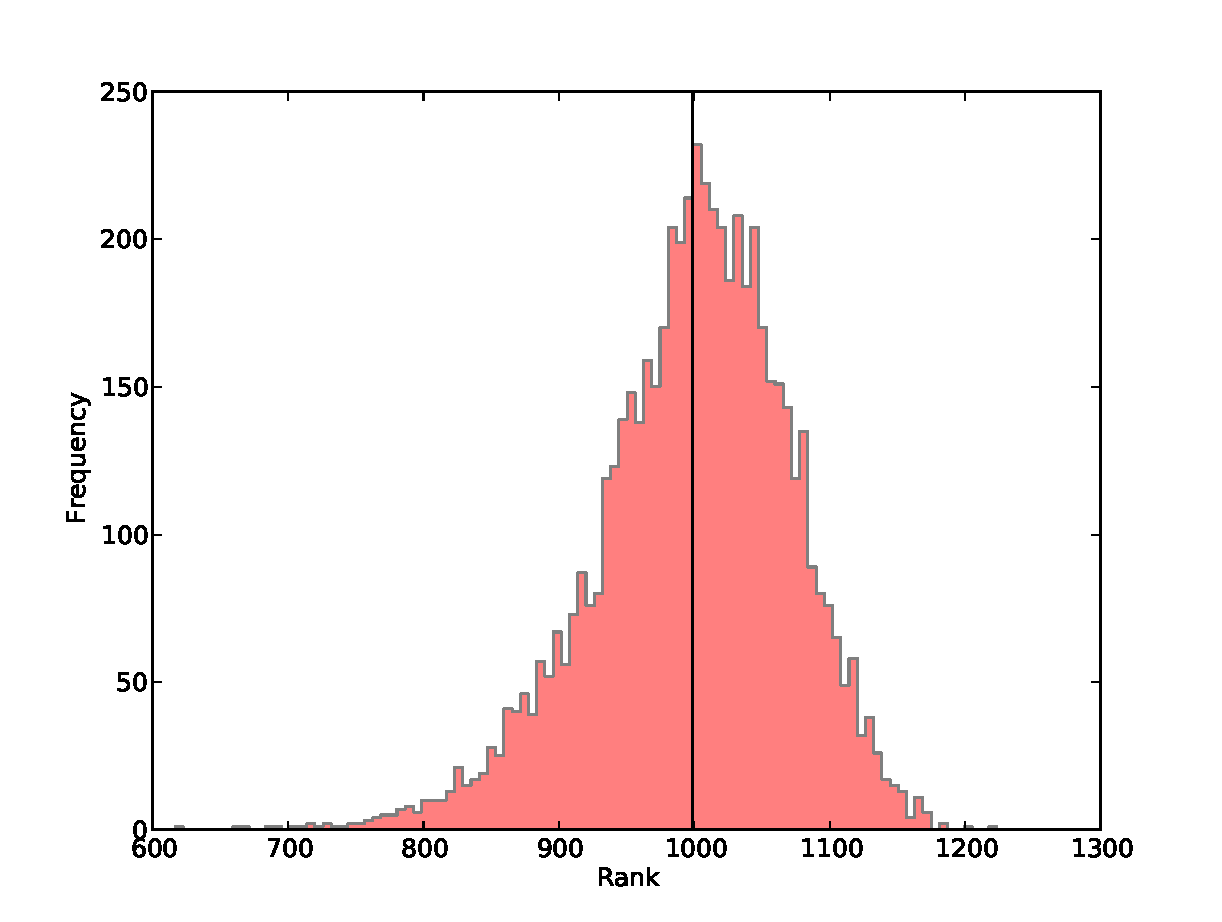
\includegraphics[width=\textwidth]{./images/realFirstLookNormal.pdf}
%        	\caption{•}
%        \end{subfigure}
%	\end{center}
%	
%	\caption{Rank histogram for real data with 2 different initialization types: (a) all 1000, (b) Gaussian with $\mu=1000$ and $\sigma=200$. Final ranks have (a) $\mu=1000$ and $\sigma=11$ and (b) $\mu=999$ and $\sigma=72$. The black vertical line marks the mean.}
%	\label{fig:firstLook}
%\end{figure}
%Next, the number of reruns were increased to 10. It was observed that the mean would drift linearly to the left. The Gaussian cutoff rule should be more careful than the 90\% rule in cutting out legitimate data. It then appears that the deeper cause of the drift is cutting out data from calculations of MT, ST, MP and SP while still assigning points to all racers. Repeating the run but this time not giving points to the outliers removed the drift previously observed.\\
%Another observed issue was the shrinking of the standard deviation of all ranks. This was accompanied by a small and decreasing drift of the mean to the right (previously it was to the left). If the system is trying to reach a steady state, the decrease of standard deviation means that any changes to rank also become smaller. Thus a lower limit on SP was imposed.
%[forgot to talk about max individual stds! those level off. individual rank changes also seem to level off. [without lower SP limit everything still falls to the floor]] [need to talk about the convergence, ie max/avg rank change] 
%objective achieved?
%summary of main results
%significance, relevance, confidence (of/in results)
%future work

\section{Conclusion}
This section should summarise the results obtained, detail
conclusions reached, suggest future work, and changes that you would make if you repeated the
experiment. This section should in general be short, 100 to 150 words
being typical for most projects.
\par\noindent
If you have opted to have multiple {\bf Theory, Method, Results}
sections, draw all the results together in a {\bf single} conclusion.

 

\section{References}

Don't forget this section. Detail the relevant references which
should be cited at the correct place in the text of the report. There
are no fixed rules as to how many references are {\it needed}. Generally
the longer the project, and the more background reading you had to do,
the more references will be required. 

When you cite a reference you must give sufficient information. For
example, for a journal article give, {\it Author}, {\it Title of
article},
{\it Journal Name}, {\it Volumn}, {\it Page}, and {\it Year}, 
while for a book give, {\it Author}, {\it Title},
{\it (Editor if there is one)}, {\it Publisher}, and {\it Year}.        
\appendix
\section{Appendices}

Material that is useful background to the report, but is not essential,
or whose inclusion within the report  would detract from its
structure and readablity, should be included in appendices. Typical
material could be diagrams of electronic circuits built, specialist
data tables used to analyse results, details of computer programs
written for analysis and display of results, photographic plates,
and, for computational projects, a copy of all written code.

Again be selective. The appendix is {\bf not} an excuse for you to add every
last detail and piece of data, but should be used to assist the reader
of the report by supplying additional material. Not all reports require
appendices and if the report is complete without this additional
material leave it out.

\end{document}
